\documentclass[a4paper,12pt]{article}
\usepackage[utf8]{vietnam}
\usepackage{hyperref}
\usepackage{graphicx}
\usepackage{xcolor}
\usepackage{subfigure}
\usepackage{float}
\usepackage{caption}
\usepackage{placeins}
\makeatletter
\setlength{\@fptop}{0pt}
\makeatother
\hypersetup{
	pdfborder = {0 0 0}
}
\title{\textbf{Báo cáo tuần 10 (P2) \\ Thực hành kiến trúc máy tính}}
\author{Họ tên: Phan Minh Anh Tuấn \\ MSSV: 20205227}
\date{}
\begin{document}
\maketitle
\tableofcontents
\newpage
\section{Assignment 3}
\subsection{Phân tích đề bài}
\textbf{Đề bài: }Create a new project, type in, and build the program of Home Assignment 3. Make the Bot run and draw a triangle by tracking \\
MarsBots là robot ảo di chuyển trong không gian hai chiều. Để điều khiển, có 5 thủ tục bao gồm: GO, STOP, TRACK, UNTRACK, ROTATE
\subsection{Triển khai MIPS}
\subsubsection{GO}
\FloatBarrier
\begin{figure}[ht!]
	\centerline{\fbox{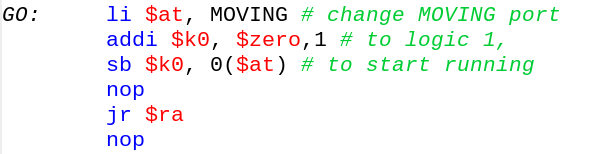
\includegraphics[width=1\textwidth]{ass3/go.png}}}
	\caption{Hàm GO}
	\label{fig:ass1}
\end{figure}
\noindent
\textbf{Trong đó: }
\begin{itemize}
	\item Tác dụng: điều khiển Marsbots bắt đầu di chuyển
	\item Cách thực hiện: đổi giá trị logic của MOVING thành 1
\end{itemize}
\FloatBarrier
\begin{figure}[ht!]
	\centerline{\fbox{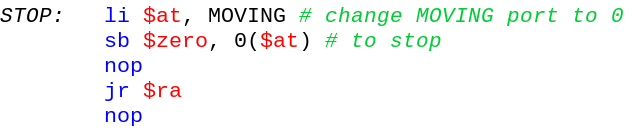
\includegraphics[width=1\textwidth]{ass3/stop.png}}}
	\caption{Hàm STOP}
	\label{fig:ass1}
\end{figure}
\clearpage
\noindent
\textbf{Trong đó: }
\begin{itemize}
	\item Tác dụng: điều khiển Marsbots dừng lại
	\item Cách thực hiện: đổi giá trị logic của MOVING thành 0
\end{itemize}
\FloatBarrier
\begin{figure}[ht!]
	\centerline{\fbox{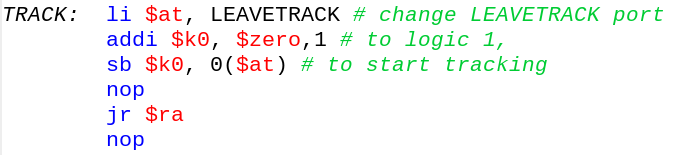
\includegraphics[width=1\textwidth]{ass3/track.png}}}
	\caption{Hàm TRACK}
	\label{fig:ass1}
\end{figure}
\noindent
\textbf{Trong đó: }
\begin{itemize}
	\item Tác dụng: điều khiển Marsbots vẽ đường thẳng
	\item Cách thực hiện: đổi giá trị logic của LEAVETRACK thành 1
\end{itemize}
\FloatBarrier
\begin{figure}[ht!]
	\centerline{\fbox{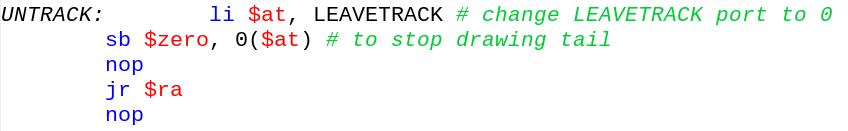
\includegraphics[width=1\textwidth]{ass3/untrack.png}}}
	\caption{Hàm UNTRACK}
	\label{fig:ass1}
\end{figure}
\noindent
\textbf{Trong đó: }
\begin{itemize}
	\item Tác dụng: điều khiển Marsbots dừng đường thẳng
	\item Cách thực hiện: đổi giá trị logic của LEAVETRACK thành 0
\end{itemize}
\newpage
\FloatBarrier
\begin{figure}[ht!]
	\centerline{\fbox{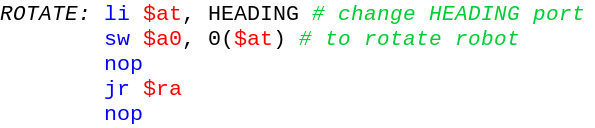
\includegraphics[width=1\textwidth]{ass3/rotate.png}}}
	\caption{Hàm ROTATE}
	\label{fig:ass1}
\end{figure}
\noindent
\textbf{Trong đó: }
\begin{itemize}
	\item Tác dụng: điều khiển Marsbots quay từ 0 - 359
	\item Cách thực hiện: đổi giá trị logic của HEADING  thành góc muốn quay. \\ Một số hướng đi phổ biến như:
	\begin{itemize}
		\item Đi lên: 0 độ
		\item Sang phải: 90 độ
		\item Đi xuống: 180 độ
		\item Sang trái: 270 độ
	\end{itemize}
\end{itemize}
\textbf{Yêu cầu: }Vẽ chữ cái đầu tiên của tên: chữ T
\begin{itemize}
	\item Cho bots đi xuống dưới (gán góc là 180 độ cho rotate)
	\item Cho bots đi sang trái (gán góc là 90 độ cho rotate)
	\item Cho bots đi xuống dưới (gán góc là 180 độ cho rotate)
	\item Đi lên, sau đó đi sang trái
\end{itemize}
\FloatBarrier
\begin{figure}[ht!]
	\centerline{\fbox{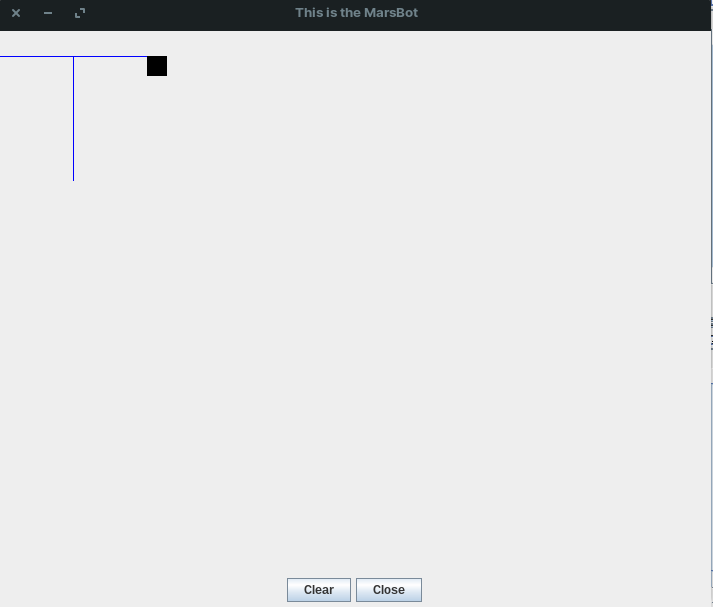
\includegraphics[width=1\textwidth]{ass3/result.png}}}
	\caption{Kết quả}
	\label{fig:ass1}
\end{figure}
\clearpage
\section{Assignment 4}
\subsection{Phân tích đề bài}
\textbf{Đề bài: }Create a new project, type in, and build the program of Home Assignment 4. Read key char and terminate the application when receiving “exit” command. \\
\subsection{Triển khai MIPS}
\FloatBarrier
\begin{figure}[ht!]
	\centerline{\fbox{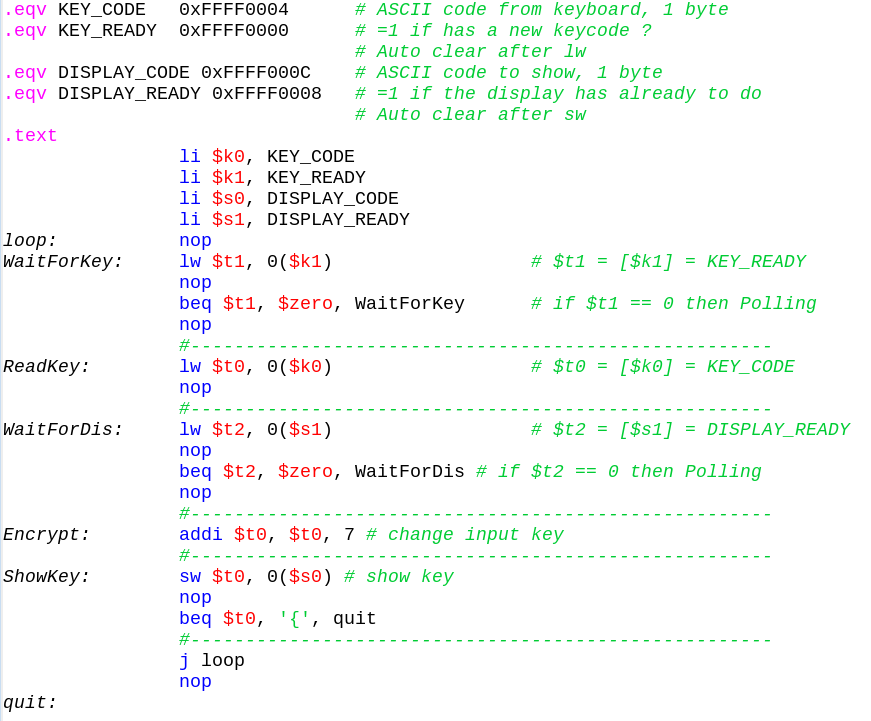
\includegraphics[width=1\textwidth]{ass4/code.png}}}
	\caption{Code bài tập 4}
	\label{fig:ass1}
\end{figure}
\noindent
Chương trình cho phép người dùng nhập vào một ký tự sau đó mã hóa nó thành một ký tự khác và hiển thị ra màn hình. Chương trình dừng lại khi nhận được kí tự "t" (Do tên là Tuấn) \\
\FloatBarrier
\begin{figure}[ht!]
	\centerline{\fbox{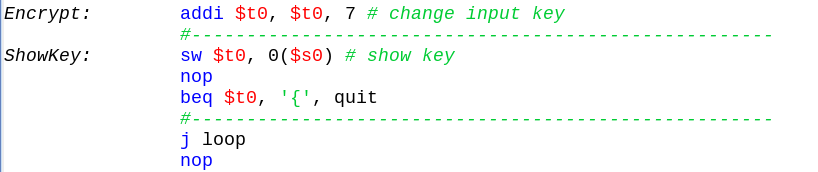
\includegraphics[width=1\textwidth]{ass4/config.png}}}
	\caption*{}
	\label{fig:ass1}
\end{figure}
\noindent
Khoảng cách mã hóa là 7 (do MSSV là 20205227), kí tự kết thúc là "t" tương ứng với "\{" khi mã hóa
\FloatBarrier
\begin{figure}[ht!]
	\centerline{\fbox{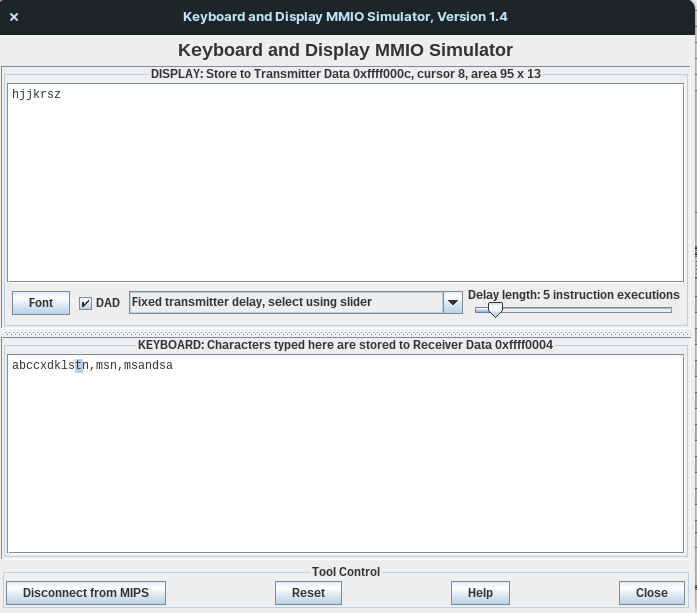
\includegraphics[width=1\textwidth]{ass4/result.png}}}
	\caption{Kết quả}
	\label{fig:ass1}
\end{figure}
\noindent
\textbf{Nhận xét: }Sau khi nhập chữ t, chương trình dừng lại không mã hóa nữa. Các kí tự được mã hóa cách 7 đơn vị trong bảng ASCII.
\end{document}